\subsection{Prototypage du premier jeu}


\subsubsection{Le concept}


\begin{wrapfigure}[15]{l}{5cm}
    \vspace{-15pt}
    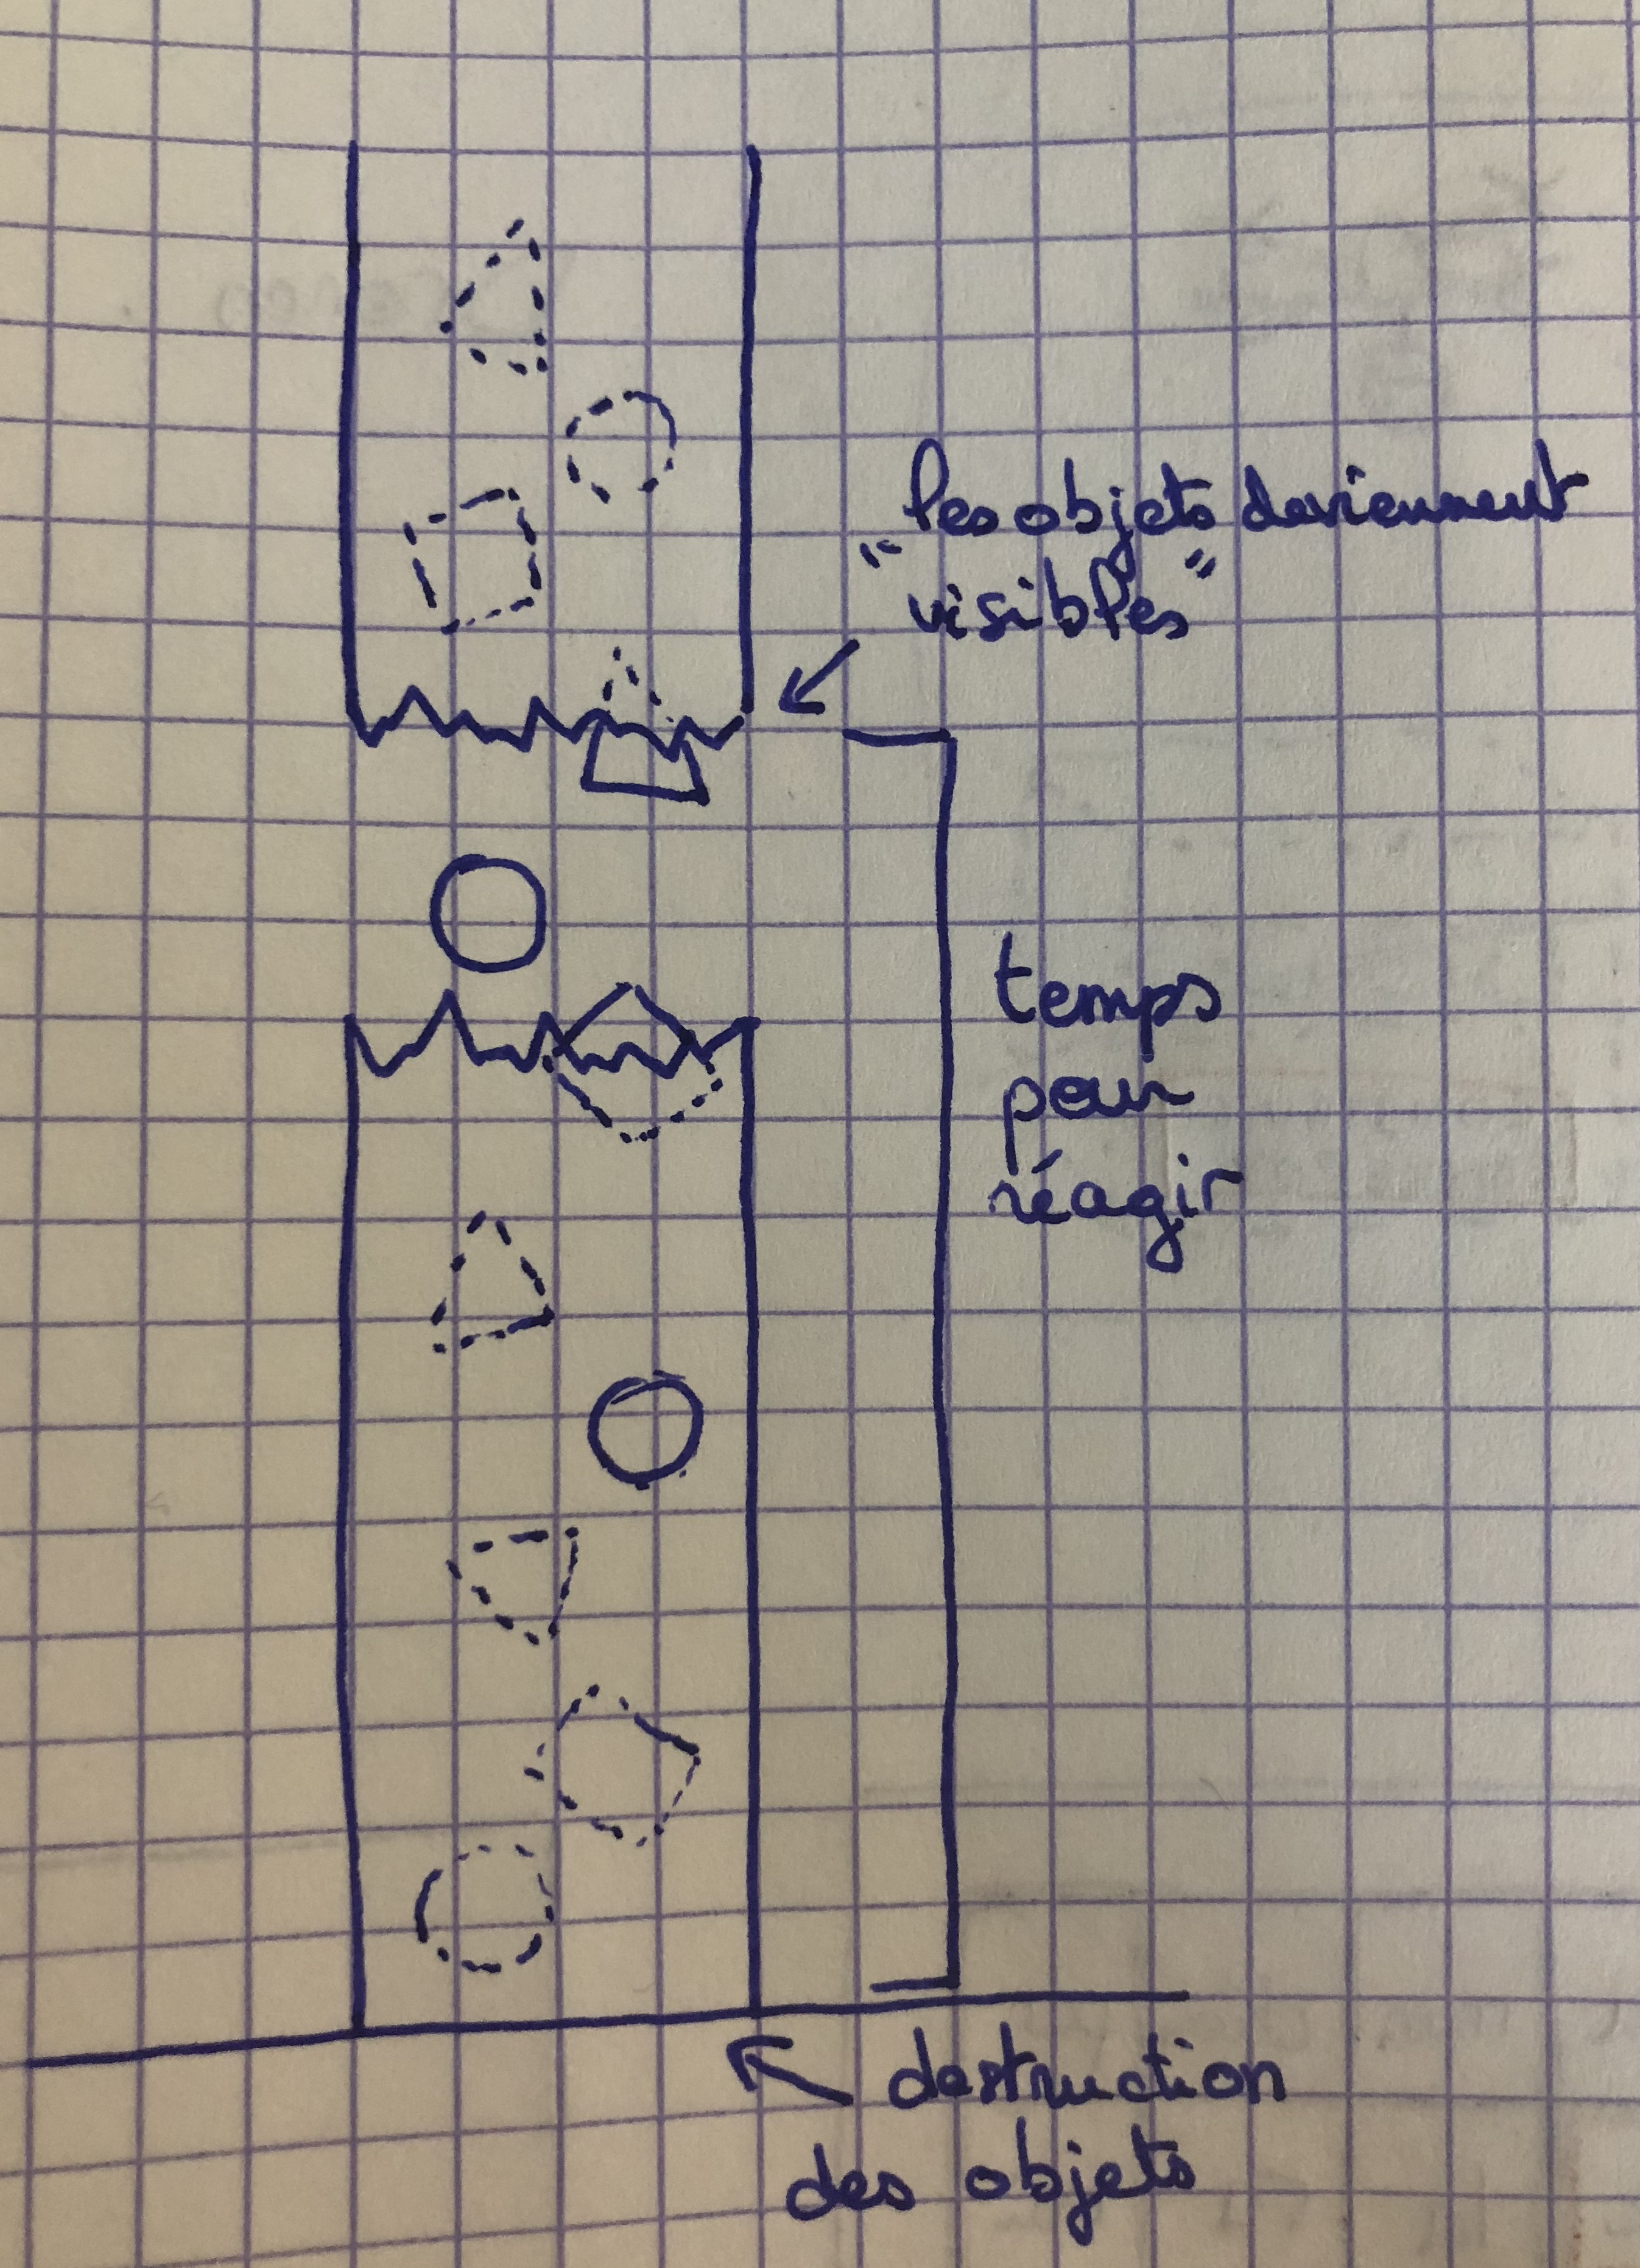
\includegraphics[width=5cm]{temps-reaction.jpg}
    \captionsetup{labelformat=simpleNumber}
    \caption{Temps de réaction}
\end{wrapfigure}

\paragraph{}Nous avons choisi le mini jeu du tuyau comme premier jeu car l'idée était plutôt simple. Il y a un tuyau au milieu de l'écran qui est brisé en son centre. Le
joueur voit des objets tomber par le trou causé par la brisure. Il doit identifier un objet cible parmi tous les autres pour l'enlever du tuyau. Pour éviter de jouer sur ses réflexes,
il faut qu'il puisse interagir avec les objets un peu de temps après qu'ils ne soient plus visibles. Pour cela, le joueur doit pouvoir interagir avec les objets qu'à partir du moment
où il peut les voir, et jusqu'à ce qu'ils soient détruits en atteignant le bas de l'écran.\\ \\

\paragraph{}A chaque fois que le joueur enlève un objet cible, ses points de score augmentent, s'il en loupe ou s'il essaie d'enlever le mauvais objet, ses points de score baissent.
Nous n'étions pas encore sûrs des conditions de victoire :
\begin{itemize}
\item Est-ce que le joueur doit atteindre un certain score avant la fin du temps ?
\item Est-ce que le joueur doit faire le meilleur score en un laps de temps imparti ?
\item Est-ce que le joueur a droit à un nombre d'erreurs maximum ?
\end{itemize}


\paragraph{}Il était également important de définir quels étaient les paramètres à régler. Dans un premier temps, nous avons pu dégager une dizaine de paramètres, certains
quantifiables, d'autres non.

Parmi les quantifiables :
\begin{itemize}
\item Vitesse d'apparition/disparition des éléments
\item Nombre de cibles total ou pourcentage de chance d'apparition de la cible durant la partie
\item Nombre de distracteurs total ou pourcentage de chance d'apparition du distracteur durant la partie
\item Emplacement des éléments par rapport au centre
\item 
\end{itemize}

\subsubsection{Création de la première scène}

\subsubsection{Amélioration du design et du gameplay}

\label{prototypage}